\section{Background}
\label{sec:background}
Before describing how \system{} works, we outline how a CDN typically operates, and what information 
it naturally has access to.  CDNs provide content caching as a service to content publishers.  A 
content publisher may wish to use a CDN provider for a number of reasons:

\begin{itemize}
\item CDNs cache content in geographically distributed locations, which allows for localized 
data centers, faster download speeds, and reduces the load on the content publisher's server.
\item CDNs typically provide usage analytics, which can help a content publisher get a better 
understanding of usage as compared to the publisher's understanding without a CDN.
\item CDNs provide a high capacity infrastructure, and therefore provide higher availability, 
lower network latency, and lower packet loss.  
\item CDNs' data centers have high bandwidth, which allows them to handle and mitigate DDoS attacks better 
than the content publisher's server.
\end{itemize}

CDN providers usually have a large number of edge servers on which content is cached; for example, 
Akamai has more than 216,000 servers in over 120 countries around the world~\cite{akamai_facts}.  
Having more edge servers in more locations increases the probability that a cache is geographically 
close to a client, and could reduce the end-to-end latency, as well as the likelihood of some kinds of 
attacks, such as BGP (Border Gateway Protocol) hijacking.  This is evident when a client requests a web page; the closest 
edge server to the client that contains the content is identified and the content is served from that 
edge server.  Most often, this edge server is geographically closer to the client than the content publisher's 
server, thus increasing the speed in which the client receives the content. If the requested page's content is 
not in one of the CDN's caches, then the request is forwarded to the content publisher's server, the CDN 
caches the response, and returns the content to the client. 

\begin{figure}[t]
\centering
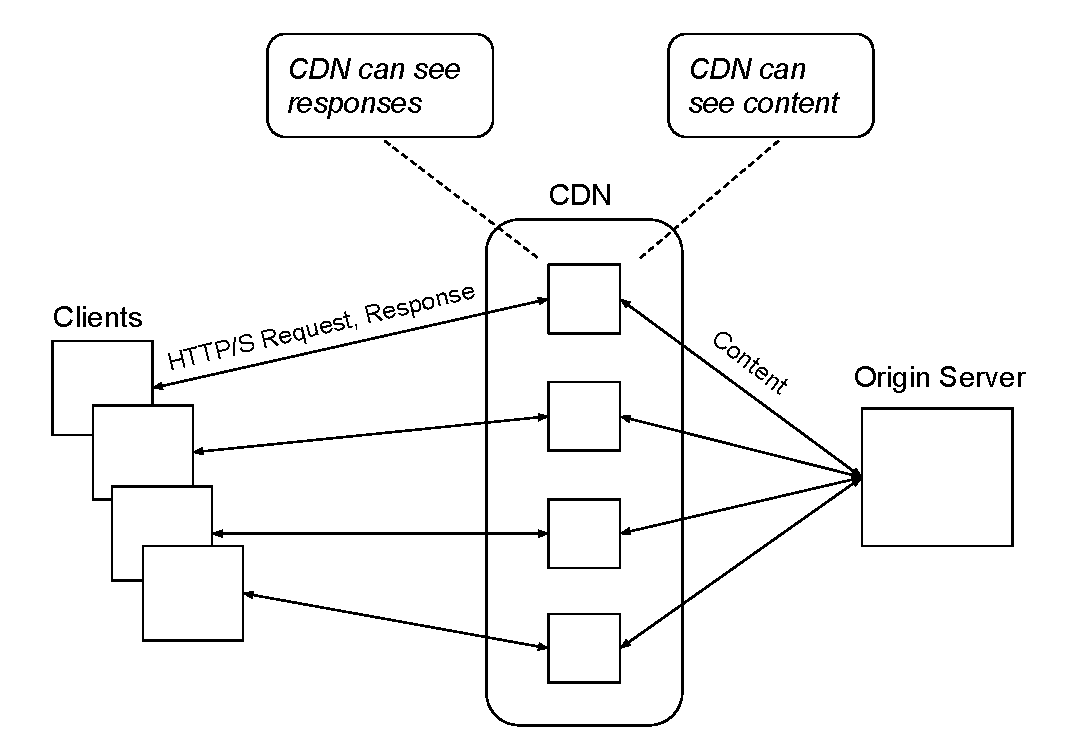
\includegraphics[width=.5\textwidth]{background_cdn}
\caption{The relationships between clients, the CDN, and content publishers in 
CDNs today.}
\label{fig:basic_cdn}
\end{figure}

Because the CDN interacts with both content publishers and clients, as shown in Figure \ref{fig:basic_cdn}, it is in a unique position 
to learn an enormous amount of information.  CDN providers know information about all clients who
access data stored at the CDN, information about all content publishers that cache content at 
CDN edge servers, and information about the content itself.

\paragraph{Knowing the content.}  CDNs, by nature, have access to all content that they distribute, as well as the 
content identifier, the URL.  First, the CDN must use the URL, which is not 
encrypted or hidden, to locate the content. Therefore, it is evident that the CDN already knows what content is 
stored in its caches.  And because CDNs provide analytics to content publishers, they keep track of cache hit 
rates, and how often content is accessed.  But the CDN does not just know about the content identifier, it also 
has access to the plaintext content.  The CDN performs optimizations on the content to increase performance; 
for example, CDNs minimize CSS, HTML, and JavaScript files, which reduces file sizes by about 20\%.  They can 
also inspect content to conduct HTTPS re-writes; we discuss how \system{} handles these types of optimizations later 
in Section \ref{sec:optimizations}. In addition, requesting content via HTTPS does not hide any information 
from the CDN; if a client requests a web page over HTTPS, the CDN terminates the TLS connection on behalf of the 
content publisher.  This means that not only does the CDN know the content, the content identifier, but also knows 
public and private keys, as well as certificates associated with the content it caches.  

Recently, the fact that CDNs 
know the content they are distributing has made its way into the legal system.  A court order was given to Cloudflare 
that required the CDN to search out and block publishers who use a variation of a trademark held by a group of 
music labels~\cite{eff_cloudflare_trademark}.  Originally, the music labels went after the trademark infringing 
website, but later the order was extended to Cloudflare; the order ``required CloudFlare to block all of its customers 
from using domain names that contained `grooveshark,' regardless of whether those domains contained First 
Amendment-protected speech, or had any connection with the `New Grooveshark' defendants who were the 
targets of the actual lawsuit.'' CDNs may also run the risk of running afoul of
copyright law: for example, recent developments in the European Union propose to
remove safe harbor protections for some CDNs if they do not employ automated detection
techniques for removing copyrighted content~\cite{eu-copyright}.
These cases highlight a key problem that CDNs face by knowing all
the content
that they distribute: it may burden them with the legal responsibility for the actions of their customers 
and clients.

\paragraph{Knowing client information.} Clients fetch content directly from the CDN's edge servers, which reveals 
information about the client's location and what the client is accessing.  Unique to CDNs is the fact that 
they can see each client's cross site browsing patterns.  CDNs host content for many different publishers, which allows 
them to see content requests for content published by different publishers.  This gives an enormous amount of 
knowledge to CDNs; for example, Akamai caches enough content around the world to see up to 30\% of global Internet 
traffic~\cite{akamai_global_traffic}.  And we have seen the implications of a CDN knowing this much information when Cloudflare 
went public with the years-long National Security Letters they had received~\cite{cloudflare_nsl}. These National Security Letters 
demand information collected by the CDN and also include a gag order, which prohibits the CDN from publicly announcing 
the information request.  

\paragraph{Knowing content publisher information.} A CDN must know information
about their customers, the content
publishers; the CDN keeps track of who the content publisher is and 
what the publisher's content is.  The combination of the CDN seeing all content in plaintext and the content's 
linkability with the publisher, gives the CDN even more power.  Additionally, as mentioned previously, the CDN often 
holds the publisher's keys (including the private key!), and the publisher's certificates.  This has led to doubts 
about the integrity of content because a CDN can impersonate the publisher from the client's point of view~\cite{levy2015stickler}.

%Because the CDN distributes content across many servers, it needs a way to direct the client 
%to the edge server that contains the correct content.  There are two different techniques commonly used 
%today to do so: 1) DNS redirection and 2) anycasting. DNS redirection occurs when the authoritative DNS 
%server receives the DNS request from the client (after locally resolving the domain), and redirects the client 
%to the correct edge server by responding with the IP address of the edge server that holds the correct content. Certain 
%optimizations can be made in selecting an edge server in the case that there are multiple edge servers 
%with cached copies of the content; these optimizations can be made based on availability, location, and 
%network conditions~\cite{krishnamurthy2001use}.  Whereas DNS redirection relies on the client's local DNS 
%resolver, and makes assumptions about where a client is from the location of the local DNS resolver, 
%anycast does not.  When anycast is used, the CDN's DNS resolver returns a set of IP addresses that 
%are on the most-preferred BGP (Border Gateway Protocol) path between the client's ISP and the CDN's 
%edge servers that announce the prefix associated with the requested domain.

%The CDN tries to serve content directly from its edge servers (unless the content is not currently 
%cached).  As a result, if a client requests a web page over HTTPS, the CDN terminates the TLS 
%connection.  Despite this practice, CDN providers are taking measures to increase the security of 
%their networks.  Akamai has established the Akamai Secure Content Delivery Network, which runs separately 
%from the rest of Akamai's systems~\cite{akamai_ssl}.  It was developed to comply with the Payment Card Industry Data
%Security Standards, and while it does comply with these standards, Akamai still essentially acts as a 
%Man in the Middle and intercepts (and terminates) the SSL session.  More recently, Cloudflare has 
%introduced Keyless SSL, which allows TLS keys to be stored on machines administered by the content 
%publishers~\cite{cloudflare_keyless}.  Unfortunately, Cloudflare will still be able to access the decrypted 
%content before it is sent to the client.

%\subsection{Cross-Border Data Storage}
%\label{sec:legal}
  

%While government access of data at a CDN could compromise a client's privacy, it becomes a more complex issue when the data being cached is geographically 
%distributed. This is clearly illustrated in the following example.  There is a content publisher in 
%country X, and she's a customer of a CDN, so her content is replicated at cache nodes in many 
%different countries.  The CDN is headquartered 
%in country Y and operates cache nodes around the world.  In this scenario it is not clear which government can ask the CDN for information; for 
%example, a government adversary may wish to learn the identity of the owner of the content, or which clients are accessing 
%this content.  Country X could demand the information of the CDN by arguing that the content is originating 
%from their country; Country Y could argue for the access to the data by stating that the CDN falls under their 
%law.  Lastly, another country may request the information because the content is replicated and stored within 
%their country.  The fact that CDNs distribute content and store it around the world opens the possibility of 
%many governments demanding access to publisher and client information.


